\documentclass{beamer}

\mode<presentation> {

%\usetheme{default}
%\usetheme{AnnArbor}
%\usetheme{Antibes}
%\usetheme{Bergen}
%\usetheme{Berkeley}
%\usetheme{Berlin}
%\usetheme{Boadilla}
%\usetheme{CambridgeUS}
%\usetheme{Copenhagen}
%\usetheme{Darmstadt}
%\usetheme{Dresden}
%\usetheme{Frankfurt}
%\usetheme{Goettingen}
%\usetheme{Hannover}
%\usetheme{Ilmenau}
%\usetheme{JuanLesPins}
%\usetheme{Luebeck}
\usetheme{Madrid}
%\usetheme{Malmoe}
%\usetheme{Marburg}
%\usetheme{Montpellier}
%\usetheme{PaloAlto}
%\usetheme{Pittsburgh}
%\usetheme{Rochester}
%\usetheme{Singapore}
%\usetheme{Szeged}
%\usetheme{Warsaw}


%\usecolortheme{albatross}
%\usecolortheme{beaver}
%\usecolortheme{beetle}
%\usecolortheme{crane}
%\usecolortheme{dolphin}
%\usecolortheme{dove}
%\usecolortheme{fly}
%\usecolortheme{lily}
%\usecolortheme{orchid}
%\usecolortheme{rose}
%\usecolortheme{seagull}
%\usecolortheme{seahorse}
%\usecolortheme{whale}
%\usecolortheme{wolverine}

%\setbeamertemplate{footline} % To remove the footer line in all slides uncomment this line
%\setbeamertemplate{footline}[page number] % To replace the footer line in all slides with a simple slide count uncomment this line

%\setbeamertemplate{navigation symbols}{} % To remove the navigation symbols from the bottom of all slides uncomment this line
}

\usepackage{graphicx} % Allows including images
\usepackage{booktabs} % Allows the use of \toprule, \midrule and \bottomrule in tables
\usepackage{amsfonts}
\usepackage{mathrsfs, bbold}
\usepackage{amsmath,amssymb,graphicx}
\usepackage{mathtools} % gather
\usepackage[export]{adjustbox} % right-aligned graphics

%----------------------------------------------------------------------------------------
%	TITLE PAGE
%----------------------------------------------------------------------------------------

\title["12"]{12: Computationally Efficient Markov chain Simulation}

\author{Taylor} 
\institute[UVA] 
{
University of Virginia \\
\medskip
\textit{} 
}
\date{} 

\begin{document}
%----------------------------------------------------------------------------------------

\begin{frame}
\titlepage 
\end{frame}

%----------------------------------------------------------------------------------------
\begin{frame}
\frametitle{Introduction}

We mention:
\begin{enumerate}
\item an example where adding auxiliary variables increases computational efficiency
\item a few tuning tips for Random-Walk Metropolis-Hastings
\item Metropolis-adjusted Langevin Algorithm (MALA)
\item Hamiltonian Monte Carlo (HMC)
\item Pseudo-Marginal Metropolis-Hastings (PMMH).
\end{enumerate}


\end{frame}


%----------------------------------------------------------------------------------------
\begin{frame}
\frametitle{Example: Data Augmentation}

\begin{itemize}
\item $y_1, \ldots, y_n \mid \mu, \sigma^2 \overset{\text{iid}}{\sim} t_{\nu}(\mu, \sigma^2)$
\item $\nu$ is assumed known
\item $p(y_i \mid \mu, \sigma^2) \propto \left(1 + \frac{1}{\nu}\left(\frac{y_i - \mu}{\sigma} \right)^2 \right)^{-(\nu+1)/2}$
\item $p(\mu) \propto 1$
\item $p(\sigma^2) \propto (\sigma^2)^{-1}$ (uniform for $\log \sigma$)
\end{itemize}
\pause

Normally we would do
$$
p(\mu, \sigma \mid y) \propto p(y \mid \mu, \sigma^2)p(\mu)p(\sigma^2)
$$
\newline

\end{frame}

%----------------------------------------------------------------------------------------
\begin{frame}[fragile]
\frametitle{Example: Data Augmentation}

Gibbs sampler not available :( 

\begin{center}
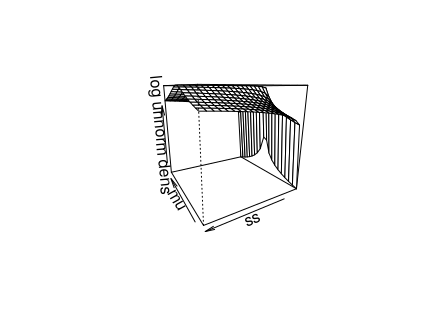
\includegraphics[width=100mm]{surf1}
\end{center}
see \verb|t_visualization.r|

\end{frame}


%----------------------------------------------------------------------------------------
\begin{frame}
\frametitle{Data Augmentation: Option 1}

Instead, we introduce $V_i$ (hidden/latent/unobserved data):
\begin{itemize}
\item $\nu$ is assumed known still
\item $p(\mu) \propto 1$ still
\item $p(\sigma^2) \propto (\sigma^2)^{-1}$ (uniform for $\log \sigma$) still
\end{itemize}

\begin{gather}
p(y_i \mid V_i, \mu, \sigma^2) = (2\pi V_i)^{-1/2} \exp\left[- \frac{1}{2 V_i}\left(y_i - \mu \right)^2 \right] \\
p( V_i \mid \sigma^2) = \frac{(\nu/2)^{\nu/2}}{\Gamma(\nu/2) }\sigma^{\nu} V_i^{-(\nu/2 + 1)}\exp\left[- \nu \sigma^2/(2 V_i) \right]
\end{gather}


Homework: show $p(y_i \mid \mu, \sigma^2)$ is the same as before.
\end{frame}



%----------------------------------------------------------------------------------------
\begin{frame}
\frametitle{Data Augmentation: Option 1}

Homework question: verify all of these:
\begin{enumerate}
\item $V_i \mid \mu, \sigma^2, y \sim \text{Inv-}\chi^2\left(\nu + 1, \frac{ \nu \sigma^2 + (y_i - \mu)^2 }{\nu+1 } \right)$
\item $\mu \mid \sigma^2, V_{1:n}, y \sim \text{Normal}\left(\frac{\sum_i \frac{1}{V_i}y_i }{\sum_i \frac{1}{V_i} }, \frac{1}{ \sum_i \frac{1}{V_i} }\right)$ 
\item $\sigma^2 \mid \mu, V_{1:n}, y) \sim \text{Gamma}\left(\frac{n \nu}{2}, \frac{\nu}{2}\sum_i \frac{1}{V_i} \right)$
\end{enumerate}

\end{frame}

%----------------------------------------------------------------------------------------
\begin{frame}[fragile]
\frametitle{Data Augmentation: Option 1}

Note:
\begin{align*}
V_i \mid \mu, \sigma^2, y &\sim \text{Inv-}\chi^2\left(\nu + 1, \frac{ \nu \sigma^2 + (y_i - \mu)^2 }{\nu+1 } \right) \\
&= \text{Inv-Gamma}\left(\frac{\nu+1}{2}, \frac{ \nu \sigma^2 + (y_i - \mu)^2 }{2 }\right)
\end{align*}

\begin{center}
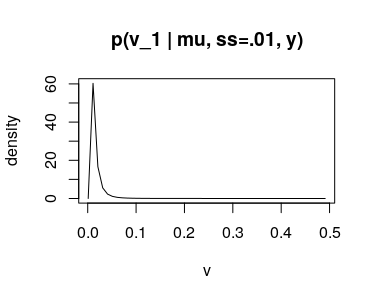
\includegraphics[width=40mm]{cond_dens_vi}
\end{center}
(see \verb|t_visualization.r|)
\newline

Near-zero values of $V_i$s lead to $\sigma^2$ being near zero, too.


\end{frame}
%----------------------------------------------------------------------------------------
\begin{frame}[fragile]
\frametitle{Data Augmentation: Option 2}

Add another parameter: $\alpha > 0$
\newline

Rename a few things:
\begin{gather}
\tau^2 = \sigma^2/\alpha^2 \\
U_i = V_i/\alpha^2 
\end{gather}

Assume a noninformative prior for $\alpha$: 
$$
p(\alpha^2) \propto (\alpha^2)^{-1}
$$

Page 295 has the full algorithm. Homework question: prove that the model is not identifiable in the full parameter space!

\end{frame}


%----------------------------------------------------------------------------------------
\begin{frame}
\frametitle{Random Walk M-H: Some Tricks}

Last section, when we were using the Metropolis-Hastings algorithm, we struggled with tuning our proposal's covariance matrix:

$$
q(\theta^* \mid \theta^{t-1}) = \text{Normal}(\theta^{t-1}, \Sigma).
$$

The book recommends setting 
$$
\Sigma \approx \frac{2.4^2}{d} \operatorname{Var}(\theta \mid y)
$$
after transforming $\theta$ be roughly normal. Here $d$ is the dimension of $\theta$. A rough approximation of the posterior covariance matrix is required.
\newline

The book also recommends aiming for an acceptance rate of about $22\%$ for problems where $d > 5$. 


\end{frame}

%----------------------------------------------------------------------------------------
\begin{frame}
\frametitle{MALA}

The {\bf Metropolis-adjusted Langevin Algorithm} is a Metropolis-Hastings algorithm with a special proposal distribution:
$$
q(\theta^* \mid \theta^{t-1}) = \text{Normal}(\theta^{t-1} + \frac{\sigma_1^2}{2} \nabla \log p(\theta \mid y) , \sigma_1^2 D).
$$
It jumps more often in the direction of the mode, and is usually more efficient than regular Random Walk Metropolis-Hastings.
\newline

Tune $\sigma_1^2 >0, D$, hopefully have an acceptance rate around ($.574$) (\href{https://pdfs.semanticscholar.org/b410/3e9b1d7e1699dd0d606b08c34394e2aff72d.pdf}{source})


\end{frame}

%----------------------------------------------------------------------------------------
\begin{frame}[fragile]
\frametitle{Pseudo-Marginal Metropolis-Hastings}

Sometimes you are not able to evaluate the likelihood at all! 
\newline

Example 1: consider a model with a lot of hidden/missing data. Here the likelihood is a high-dimensional integral or sum that may be either impossible or computationally difficult to evaluate. Examples include state space models, factors models, ``regular models" with missing data.
\newline
\pause

Example 2: you have a simple model, but too much data. Evaluating the density either takes too long to iterate through all of your observations, or the observations can't be read into memory. So, you can't do it several thousand times to run an MCMC sampler. 

\end{frame}

%----------------------------------------------------------------------------------------
\begin{frame}[fragile]
\frametitle{Pseudo-Marginal Metropolis-Hastings}

The marginal Metropolis-Hastings' acceptance ratio is
\begin{align*}
\frac{  p(y_{1:T} \mid \theta') p(\theta')}{  p(y_{1:T} \mid \theta) p(\theta) }
\frac{ q(\theta \mid \theta') }{  q(\theta' \mid \theta) },
\end{align*}

and the {\bf pseudo-marginal Metropolis-Hastings} acceptance ratio is 

\begin{align*}
\frac{ \hat{p}(y_{1:T} \mid \theta') p(\theta') }{  \hat{p}(y_{1:T} \mid \theta) p(\theta) }
\frac{ q(\theta \mid \theta') }{  q(\theta' \mid \theta) }.
\end{align*}

\end{frame}

%----------------------------------------------------------------------------------------
\begin{frame}[fragile]
\frametitle{Pseudo-Marginal Metropolis-Hastings}


Rewrite it a little differently:

\begin{align*}
\frac{ \overbrace{ \hat{p}(y_{1:T} \mid u', \theta')p(\theta') \begingroup\color{red} \psi(u' | y_{1:T},\theta')\endgroup }^{\text{unnormalized target} }}{  \hat{p}(y_{1:T}| u, \theta) p(\theta)\begingroup\color{red}\psi(u|y_{1:T},\theta)\endgroup }
\frac{ \begingroup\color{red} \psi(u|y_{1:T},\theta)\endgroup q(\theta| \theta') }{ \underbrace{ \begingroup\color{red} \psi(u'|y_{1:T},\theta')\endgroup q(\theta'| \theta)}_{\text{proposal distribution} } }
\end{align*}




\begin{itemize}
\item The full normalized target is $p(\theta,u\mid y_{1:T}) =  \frac{\hat{p}(y_{1:T}\mid u, \theta)\psi(u \mid y_{1:T},\theta)p(\theta \mid y_{1:T}) }{p(y_{1:T}\mid \theta) }$
\item When likelihood is unbiased, the marginal is $p(\theta \mid y_{1:T})$
\item $u$ is the collection of all auxiliary random variables (e.g. importance sampling output, a particle filter's samples and ancestor indices, etc.)
\end{itemize}

% special case not retaining the state samples
% -$k$ is the index of the chosen particle path.


\end{frame}



%----------------------------------------------------------------------------------------
\begin{frame}
\frametitle{HMC}

Hamiltonian Monte Carlo can be quite effective at sampling from a high-dimensional posterior. It makes use of the derivative of the log-likelihood as well. 
\newline

We will describe it in three steps: 
\begin{enumerate}
\item Describing Hamiltonian dynamics in continuous time
\item Describing how to discretize Hamiltonian dynamics
\item Describing how to use these in a proposal distribution in the Metropolis-Hastings algorithm.
\end{enumerate}

\pause
Video time! 
\begin{enumerate}
\item \url{https://www.youtube.com/watch?v=mzjErXqBXw4}
\item \url{https://www.youtube.com/watch?v=87E0DKs5bok}
\end{enumerate}

\end{frame}

%----------------------------------------------------------------------------------------
\begin{frame}
\frametitle{HMC}

Say you have $\theta_1, \ldots, \theta_d$. You add $d$ auxiliary variables: $\phi_1, \ldots, \phi_d$.
\newline

It's customary to use the notation $q_1, \ldots, q_d$ (the positions), and $p_1, \ldots, p_d$ (the momenta).
\newline
\pause

A HMC proposal follows a two-step procedure:
\begin{enumerate}
\item sample a random momentum vector
\item transform the momentum and position {\bf nonrandomly} using Hamilton's equations
\end{enumerate}
Both steps are transition kernels that preserve the stationary distribution.

\end{frame}


%----------------------------------------------------------------------------------------
\begin{frame}
\frametitle{HMC: a 1-d example}

Start with one-dimensional $q$ (position) and one-dimensional $p$ (momentum). Also, $m$ is mass (a tuning parameter).
\newline

\begin{enumerate}
\item potential energy: $U(q)$ is negative the logarithm of the unnormalized posterior.
\item kinetic energy: $K(p) = \frac{p^2}{2m}$ 
\end{enumerate}
$p =  m \times \text{velocity}$
\newline

Two good resources:
\begin{enumerate}
\item \url{https://arxiv.org/pdf/1206.1901.pdf} (primary reference), 
\item \url{https://arxiv.org/pdf/1701.02434.pdf}
\end{enumerate}

\end{frame}


%----------------------------------------------------------------------------------------
\begin{frame}
\frametitle{HMC}

When the particle goes up the hill, it loses kinetic energy, and gains potential energy. 
\newline

Define the {\bf Hamiltonian} as
$$
H(q,p) = U(q) + K(p).
$$ 

and define {\bf Hamilton's Equations} as

\begin{gather}
\frac{dq}{dt} = \frac{\partial H(q,p)}{\partial p} \\
\frac{dp}{dt} = -\frac{\partial H(q,p)}{\partial q}
\end{gather}

\end{frame}

%----------------------------------------------------------------------------------------
\begin{frame}
\frametitle{HMC: a first example}


Assume the posterior is a Gaussian with mean $y=0$ and variance $1$. Negative log of the posterior is proportional to 
$$
U(q) = \frac{q^2}{2}.
$$

Also, assume kinetic energy is of the form
$$
K(p) = \frac{p^2}{2m}.
$$
\pause
% where $p =  m \times \text{velocity}$, and 


so
\begin{gather}
\frac{dq}{dt} = \frac{\partial H(q,p)}{\partial p} =  \frac{d K(p) }{d p} = p(t)/m \\
\frac{dp}{dt} = -\frac{\partial H(q,p)}{\partial q} = -\frac{d U(q)}{d q} = -q(t)
\end{gather}

\end{frame}

%----------------------------------------------------------------------------------------
\begin{frame}
\frametitle{HMC: a first example}

If $m=1$, a solution to
\begin{gather}
\frac{dq}{dt} = \frac{\partial H(q,p)}{\partial p} =  \frac{d K(p) }{d p} = p(t) \\
\frac{dp}{dt} = -\frac{\partial H(q,p)}{\partial q} = -\frac{d U(q)}{d q} = -q(t)
\end{gather}

is


\begin{gather}
q(t) = r \cos(a + t)\\
p(t) = -r \sin(a + t)
\end{gather}


\end{frame}

%----------------------------------------------------------------------------------------
\begin{frame}
\frametitle{HMC: a first example}

For this particular model, $(q,p)'$ rotates clockwise in phase-space.
\begin{gather}
q(t) = r \cos(a + t)\\
p(t) = -r \sin(a + t)
\end{gather}
Can be written as 

$$
\left[\begin{array}{c}
r \cos(a + t) \\
-r \sin(a + t) 
\end{array}\right]
=
\underbrace{
\left[\begin{array}{cc}
\cos([t-s]) & \sin([t-s]) \\
\sin([t-s])  & \cos([t-s])
\end{array}\right]}
_{T_{t-s}}
\left[\begin{array}{c}
r \cos(a + s) \\
-r \sin(a + t) 
\end{array}\right]
$$
(use Angle-Sum trig identity)
\end{frame}

%----------------------------------------------------------------------------------------
\begin{frame}
\frametitle{HMC: a first example}

When $m \neq 1$, $T_s$ might look like this. 
\begin{center}
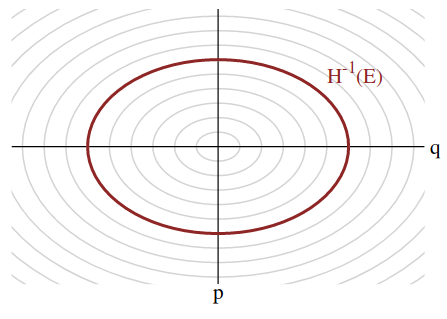
\includegraphics[width=90mm]{level_sets.png}
\end{center}
image source: \url{https://arxiv.org/pdf/1701.02434.pdf}

\end{frame}

%----------------------------------------------------------------------------------------
\begin{frame}
\frametitle{HMC}

Now assume $d$-dimensional posterior $\mathbf{q} = (q_1, \ldots, q_d)$ and $\mathbf{p} = (p_1, \ldots, p_d)$.
\newline

When
$$
K(\mathbf{p}) = \frac{\mathbf{p}'M^{-1}\mathbf{p}}{2} 
$$

Hamilton's equations become

\begin{gather}
\frac{dq_i}{dt} = \frac{\partial H(\mathbf{q},\mathbf{p})}{\partial p_i} =  \frac{d K(\mathbf{p}) }{d p_i} = [M^{-1}\mathbf{p}]_i  \\
\frac{dp_i}{dt} = -\frac{\partial H(\mathbf{q},\mathbf{p})}{\partial q_i} = -\frac{d U(\mathbf{q})}{d q_i} 
\end{gather}

Recall that $U(\mathbf{q})$ is the negative log of the posterior you're interested in.
\end{frame}


%----------------------------------------------------------------------------------------
\begin{frame}
\frametitle{Property 1: Reversibility of $T_s$}

Recall  $T_s: [\mathbf{q}(0), \mathbf{p}(0)] \mapsto [\mathbf{q}(s), \mathbf{p}(s)]$. It is always has an easy-to-find inverse.
\newline

Proof: just take the negative of the derivatives.


\end{frame}

%----------------------------------------------------------------------------------------
\begin{frame}
\frametitle{Property 2: Conservation of the Hamiltonian}

Using the chain rule:

\begin{align*}
\frac{d H}{dt} &= \sum_{i=1}^d \frac{\partial H}{\partial p_i}\frac{dp_i}{dt} + \sum_{i=1}^d \frac{\partial H}{\partial q_i}\frac{dq_i}{dt} \\
&= \sum_{i=1}^d \frac{dK}{dp_i}\frac{dp_i}{dt} + \sum_{i=1}^d \frac{dU}{dq_i}\frac{dq_i}{dt} \\
&= \sum_{i=1}^d \frac{dK}{dp_i}\left( - \frac{d U}{dq_i}\right) + \sum_{i=1}^d \frac{dU}{dq_i}\frac{dK}{dp_i} \\
&= 0
\end{align*}

Moving through time keeps you on the same contour or level-set in the phase space.
\end{frame}

%----------------------------------------------------------------------------------------
\begin{frame}
\frametitle{HMC}

$T_s$ keeps you on a level-set/contour: 
\begin{center}
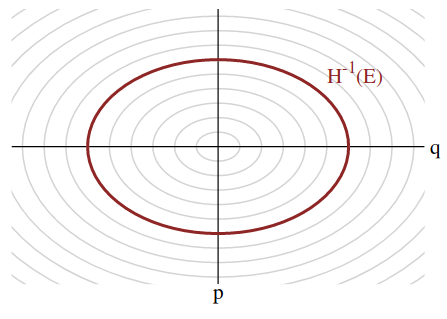
\includegraphics[width=100mm]{level_sets.png}
\end{center}
\end{frame}

%----------------------------------------------------------------------------------------
\begin{frame}
\frametitle{HMC Property 3 and 4: Volume Preservation and Symplecticness}

Volume preservation: $(q,p)$ and $T_s(q,p)$ have the same volume.
\newline

Symplecticness: a nice property of the Jacobian (matrix of time derivatives) of $T_s$.
\newline

Another thing: when we approximate these dynamics in our proposal distribution, these properties are preserved!




\end{frame}

%----------------------------------------------------------------------------------------
\begin{frame}
\frametitle{HMC: looking back at the big picture}

HMC will work as follows: given that we are currently at position $\mathbf{q}(t)$, we are going to sample a momentum vector (which puts us on one of the level-sets), and then we are going to follow $T_s$ for a deterministic amount of time (how much time is a tuning parameter we decide on).
\newline

\begin{center}
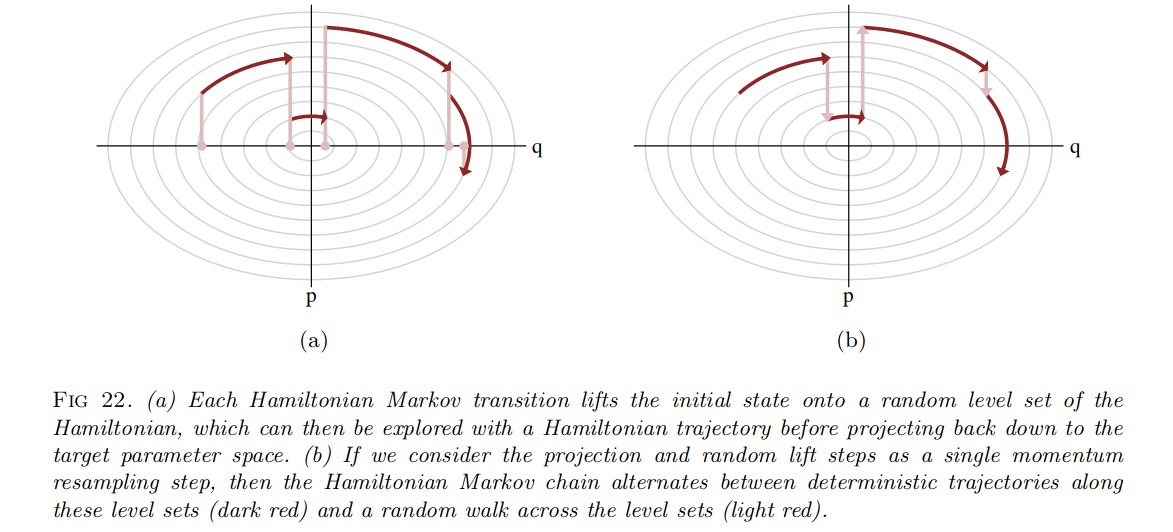
\includegraphics[width=100mm]{1d_algo_vis.png}
\end{center}
\pause

Following a contour line is impossible in continuous time though...
\end{frame}
%----------------------------------------------------------------------------------------
\begin{frame}
\frametitle{Discretizing Hamilton's Equations: Version 1.0}

We need to be able to approximate $T_s$ using the derivatives. To do that, we pick a small change in time called $\epsilon$. Then we take $L$ steps of size $\epsilon$.
\newline

Two procedures are described. The last one is the one that is most commonly used. 
\newline

For simplicity, assume the mass matrix is diagonal, making
$$
K(\mathbf{p}) = \mathbf{p}'M^{-1}\mathbf{p}  = \sum_{i=1}^d \frac{p_i^2}{2m_i}.
$$


\end{frame}

%----------------------------------------------------------------------------------------
\begin{frame}
\frametitle{Discretizing Hamilton's Equations: Version 1.0}

When $K(\mathbf{p})= \sum_{i=1}^d \frac{p_i^2}{2m_i}$, {\bf Euler's method} approximates the solution of

\begin{gather}
\frac{dq_i}{dt} = \frac{\partial H(\mathbf{q},\mathbf{p})}{\partial p_i} =  \frac{d K(\mathbf{p}) }{d p_i} = p_i/m_i  \\
\frac{dp_i}{dt} = -\frac{\partial H(\mathbf{q},\mathbf{p})}{\partial q_i} = -\frac{d U(\mathbf{q})}{d q_i} 
\end{gather}

as 
\begin{gather}
q_i(t + \epsilon) =  q_i(t ) + \epsilon p_i(t)/m_i \\
p_i(t + \epsilon) =  p_i(t) - \epsilon \frac{d U}{d q_i}(\mathbf{q}(t))  
\end{gather}


\end{frame}

%----------------------------------------------------------------------------------------
\begin{frame}
\frametitle{Discretizing Hamilton's Equations: Version 1.0}

\begin{center}
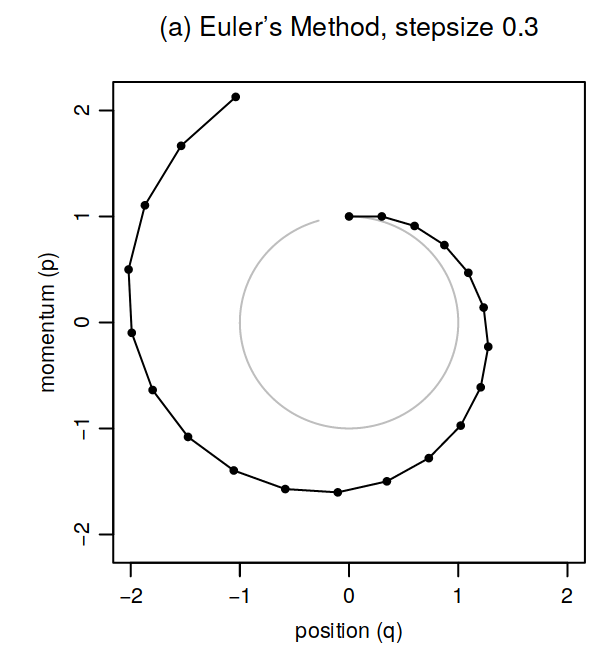
\includegraphics[width=60mm]{eulers_method.png}
\end{center}

Twenty steps when $H(q,p) = p^2/2 + q^2/2$, the initial state is $(q,p) = (0,1)$. 

\end{frame}
%----------------------------------------------------------------------------------------
\begin{frame}
\frametitle{Discretizing Hamilton's Equations: Version 2.0}

When $K(\mathbf{p})= \sum_{i=1}^d \frac{p_i^2}{2m_i}$, {\bf the leap-frog method} approximates

\begin{gather}
\frac{dq_i}{dt} = \frac{\partial H(\mathbf{q},\mathbf{p})}{\partial p_i} =  \frac{d K(\mathbf{p}) }{d p_i} = p_i/m_i  \\
\frac{dp_i}{dt} = -\frac{\partial H(\mathbf{q},\mathbf{p})}{\partial q_i} = -\frac{d U(\mathbf{q})}{d q_i} 
\end{gather}

with
\begin{gather}
p_i(t + \epsilon/2) =  p_i(t) - (\epsilon/2) \frac{d U}{d q_i}(\mathbf{q}(t)) \\
q_i(t + \epsilon) = q_i(t ) + \epsilon \frac{p_i(t+\epsilon/2)}{m_i} \\
p_i(t + \epsilon) =  p_i(t + \epsilon/2) - (\epsilon/2) \frac{d U}{d q_i}(\mathbf{q}(t+\epsilon)) 
\end{gather}


\end{frame}

%----------------------------------------------------------------------------------------
\begin{frame}
\frametitle{Discretizing Hamilton's Equations: Version 2.0}

\begin{center}
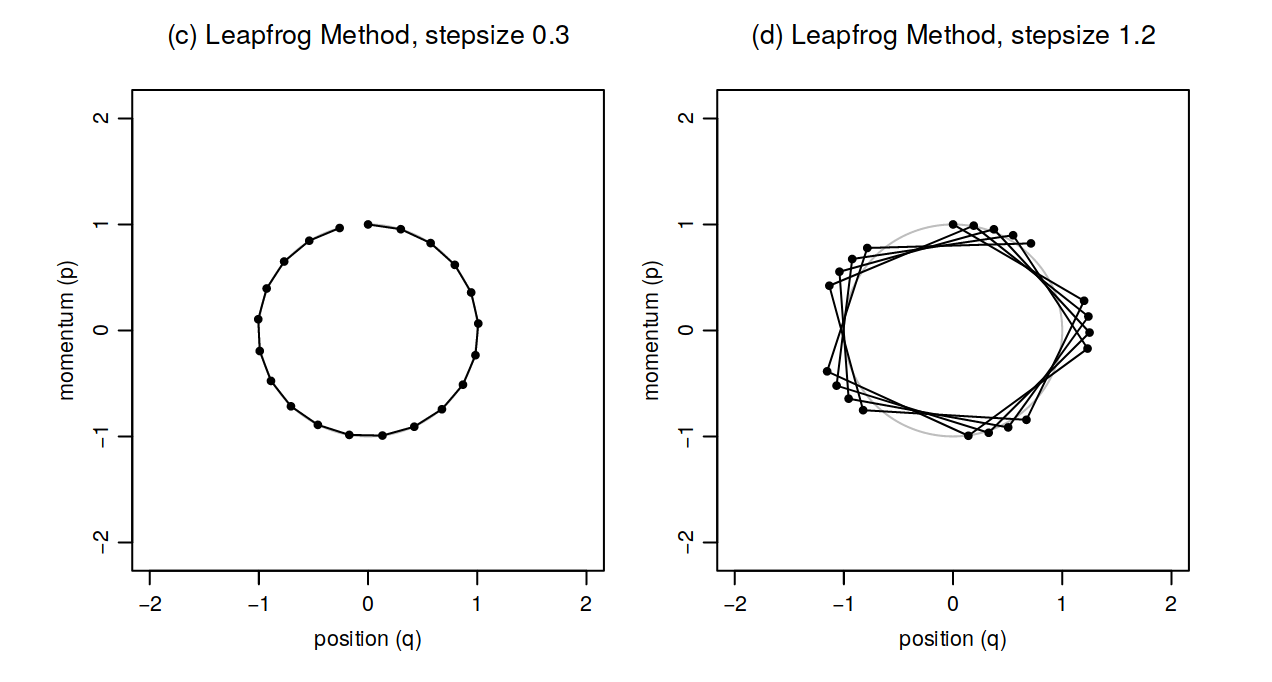
\includegraphics[width=120mm]{leapfrog_method.png}
\end{center}

Twenty steps when $H(q,p) = p^2/2 + q^2/2$, the initial state is $(q,p) = (0,1)$.

\end{frame}
%----------------------------------------------------------------------------------------
\begin{frame}
\frametitle{Describing the HMC algorithm}

The algorithm targets the distribution for $(\mathbf{q}, \mathbf{p})$:
\begin{align*}
\frac{1}{Z}\exp\left[-\frac{H(\mathbf{q}, \mathbf{p})}{T} \right] &= \frac{1}{Z}\exp\left[-\frac{K(\mathbf{p}) + U(\mathbf{q})}{T} \right] \\
&= \frac{1}{Z}\exp\left[-\frac{K(\mathbf{p})}{T} \right]\exp\left[-\frac{U(\mathbf{q})}{T}\right] \\
&= \frac{1}{Z}\exp\left[-\frac{K(\mathbf{p})}{T} \right] \times \\
&\hspace{10mm} \exp\left[-\frac{-\log\{\text{prior}(\mathbf{q}) \times \text{likelihood}(\mathbf{q}) \}  }{T}\right] 
\end{align*}


\end{frame}

%----------------------------------------------------------------------------------------
\begin{frame}
\frametitle{Describing the HMC algorithm}

Step 1: 
\newline

Sample $p$ from the conditional target distribution
$$
\frac{1}{Z}\exp\left[-\frac{K(\mathbf{p})}{T} \right].
$$
In our case, this is the same as the marginal, due to independence.
\newline

Notice how this is a Gibbs-like step! It preserves the stationary distribution, and it has $100$\% chance of being accepted.


\end{frame}

%----------------------------------------------------------------------------------------
\begin{frame}
\frametitle{Describing the HMC algorithm}

Step 2: 
\newline

If we could integrate Hamilton's equations exactly, then our proposal would be deterministic, and we would accept with probability $1$, because the Hamiltonian is preserved (property 2). 
\newline

However, because we are using numerical leap-frog integration, there will be some change in the Hamiltonian. We think of the $L$ leap-frog steps as a proposal distribution. This is a deterministic proposal, and it's symmetrical (we don't prove this). So what we end up with is a Metropolis-like acceptance probability:
$$
\min\left[1, \frac{\exp\left[ -H(\mathbf{q}^*,\mathbf{p}^*) \right]}{\exp\left[ -H(\mathbf{q},\mathbf{p}) \right] } \right]
$$



\end{frame}

%----------------------------------------------------------------------------------------
\begin{frame}[fragile]
\frametitle{Describing the HMC algorithm}

Code from \url{https://arxiv.org/pdf/1206.1901.pdf} that performs one iteration of HMC can be found in the file \verb|hmc.r|.
\newline

Here's a visualization:\\
\url{https://chi-feng.github.io/mcmc-demo/}


\end{frame}





\end{document} 
